\documentclass[a4paper, 10pt]{article}
\usepackage{moderntex}


\title{Numerical Solution of Differential Equations\\by Difference Methods}
\author{Trym Sæther}
\date{\today}
\begin{document}

\sloppy

\maketitle
\tableofcontents
\newpage

\chapter{Finite Difference Method (FDM)}
FDM er en numerisk metode for å løse ODE og PDE ved å diskretisere domenet og tilnærme den deriverte med differanser.

\section{Teori}
\subsection{Taylors formel}
\begin{theorem}{Taylor-rekke for to variabler}{taylor}
	La \(u_m^{n} = u(x_m, t_n) \approx u(x, t)\) være approksimasjonen av den eksakte løsningen \(u\) i punktet \((x_m, t_n)\).
	\begin{align} \label{eq:taylor}
		u_{m+1}^{n+1} &= \sum_{i=0}^{p} \frac{1}{i!} \left(h \partial_x + k \partial_t\right)^i u(x, t) + r_{p+1}(x, t) \tag{taylor} \\
		r_p & = \frac{1}{(p+1)!} \left(h \partial_x + k \partial_t\right)^{p+1} u(x, t) \tag{rest}
	\end{align}
	der \(h, k\) er steglengdene i \((x, t)\) og \(p\) er ordren til Taylor-rekken.
\end{theorem}
\begin{remark*}{Uniform Gridstørrelse}{}
	Hvis vi har en uniform gridstørrelse \(\mathbb{G}\) i \(x\) og \(t\), kan vi skrive:
	\[\mathbb{G} = \{(x_m, t_n) \mid x_m = x_0 + mh, t_n = t_0 + nk \text{ for } m = 0, 1, \ldots, M \text{ og } n = 0, 1, \ldots, N\}\]
	der \(h\) er steglengden i \(x\) og \(k\) er steglengden i \(t\).
\end{remark*}

\section{Motivasjon}
Gitt en vilkårlig differensiallikning (ODE), som f.eks. \( \ddn[f(x)]{2}{x} = f(x) - x^3 \)\label{eq:ode} med randbetingelser: \( f(x_0) = \alpha \) og \( f(x_N) = \beta \).
Denne ODE har allerede en eksakt løsning: \( f(x) = c_0e^x + c_1e^{-x} + x^3 + 6x \)\label{eq:exact}.
Men, hva om vi ikke har en eksakt løsning? Da kan vi bruke FDM til å tilnærme løsningen.

\section{FDM-oppskrift}
\begin{enumerate}
	\item \textbf{Diskretisering:} Del intervallet \(x \in [\alpha, \beta]\) inn i \(N\) like store delintervaller med \(x_i = \alpha + ih\) for \(i = 0,1,\ldots,N\) og \(h = 2/N\)
	\item \textbf{Taylor-utvikling:} Rekkeutvikle \(f(x \pm h)\) rundt \(x\).
	\item \textbf{Differanse metoder:} Finn en lineærkombinasjon av \(f(x \pm h)\) som tilnærmer den deriverte.
	      \begin{align}
		      C_{-1}f(x - h) + C_0f(x) + C_1f(x + h)   & = \ddn[f(x)]{2}{x} + \mathcolor{blue}{O(h)} \tag{Central} \label{eq:center}    \\
		      C_{0}f(x) + C_1f(x + h ) + C_2f(x + 2h)  & = \ddn[f(x)]{2}{x} + \mathcolor{blue}{O(h^2)} \tag{Forward} \label{eq:forward} \\
		      C_{-2}f(x - 2h) + C_{-1}f(x-h) + C_0f(x) & = \ddn[f(x)]{2}{x} + \mathcolor{blue}{O(h)} \tag{Backward} \label{eq:backward}
	      \end{align}
	\item \textbf{Diskretiser og løs ODE:} Anvend en av disse metodene, f.eks. \ref{eq:center} på \ref{eq:ode} og løs ligningssettet \(T_h \vec{f} = \vec{b}\), hvor \(T_h\) er en tri-diagonal.
\end{enumerate}

\section{Differanseoperatorer}

Differanseoperatorer er diskrete tilnærminger av deriverte og kan brukes til å konstruere differanseskjemaer for numerisk løsning av \gls{ode} og \gls{pde}.

Differanseoperatorer er fundamentale byggeklosser for diskretisering av deriverte, og danner grunnlaget for numeriske metoder for differensiallikninger.

\subsection{Fremover differanseoperator}
\begin{definition}{Fremover differanse}{}
	\begin{equation}
		\Delta_h u(x) = u(x + h) - u(x) \label{eq:forward_diff}
	\end{equation}
	der $h > 0$ er steglengden.
\end{definition}

\begin{remark*}{}{}
	Fremover differanse tilnærmer den første deriverte med nøyaktighet $O(h)$:
	\begin{equation}
		\frac{\Delta_h u(x)}{h} = u'(x) + \frac{h}{2}u''(x) + O(h^2)
	\end{equation}
\end{remark*}

\subsection{Bakover differanseoperator}
\begin{definition}{Bakover differanse}{}
	Bakover differanseoperatoren er definert som:
		\begin{align*}
			\nabla_h u(x) & = \frac{1}{h} \left( u(x) - u(x - h) \right) \tag{bakover} \\
			r_1(x) & = \frac{h}{2}u''(x) + O(h^2) \tag{rest}
		\end{align*}
		der \(h > 0\) er steglengden og \(r_p\) er restleddet.
	\end{definition}
\begin{remark*}{}{}
	Bakover differanse tilnærmer også den første deriverte med nøyaktighet $O(h)$, men bruker tidligere punkter:
	\begin{equation}
		\frac{\nabla_h u(x)}{h} = u'(x) - \frac{h}{2}u''(x) + O(h^2)
	\end{equation}
\end{remark*}

\begin{example}{}{}
	\( f''(x) = f(x) - x^3 \) med \( [f(0), f(2)] = [0, 20] \) og \( N = 5 \). Det gir 1D FDM-ligningssettet med sentral differanseoperator:
	\begin{align*}
		\overbrace{
			\begin{bmatrix}
				1             & 0                  & 0             & \cdots & 0             \\
				\frac{1}{h^2} & -\frac{2}{h^2} - 1 & \frac{1}{h^2} & \cdots & 0             \\
				0             & \ddots             & \ddots        & \ddots & \vdots        \\
				\vdots        & \ddots             & \ddots        & \ddots & \frac{1}{h^2} \\
				0             & \cdots             & 0             & 0      & 1
			\end{bmatrix}}^{L_h}
		\overbrace{
			\begin{bmatrix}
				f(x_0) \\ f(x_1) \\ \vdots \\ f(x_{N-1}) \\ f(x_N)
			\end{bmatrix}}^{\vec{f}}
		            & =
		\overbrace{
		\begin{bmatrix}
				\alpha \\ h^2(x_1^3 - x_1) \\ \vdots \\ h^2(x_{N-1}^3 - x_{N-1}) \\ \beta
			\end{bmatrix}}^{\vec{b}} \\
		L_h \vec{f} & = \vec{b}\tag{SUS!}
	\end{align*}

	\vspace{0.5em}

	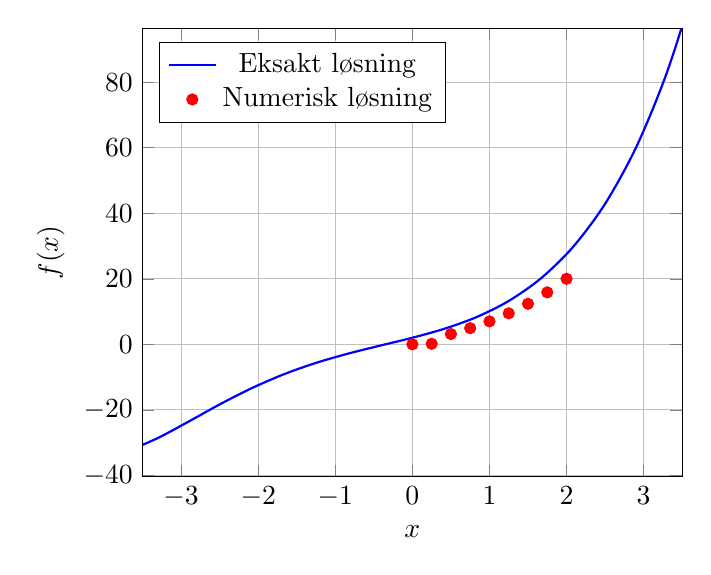
\begin{tikzpicture}
		\begin{axis}[
				xlabel={\(x\)},
				ylabel={\(f(x)\)},
				grid=major,
				legend pos=north west,
				xmin=-3.5,
				xmax=3.5,
				xtick={-3, -2, -1, 0, 1, 2, 3},
			]
			\addplot[smooth, thick, blue] {x^3 + 6*x + exp(x) + exp(-x)};
			\addplot[only marks, red] coordinates {
					(0, 0)
					(0.25, 0.1516)
					(0.5, 3.125)
					(0.75, 4.922)
					(1, 7)
					(1.25, 9.453)
					(1.5, 12.375)
					(1.75, 15.859)
					(2, 20)
				};
			\legend{Eksakt løsning, Numerisk løsning}
		\end{axis}
	\end{tikzpicture}
	\label{fig:ode}
\end{example}

\subsection{Sentral differanseoperator}
\begin{definition}{Sentral differanse}{}
	\begin{equation}
		\delta_h u(x) = u(x + h/2) - u(x - h/2) \label{eq:central_diff}
	\end{equation}
\end{definition}

\begin{remark*}{}{}
	Sentral differanse gir en mer nøyaktig tilnærming av den første deriverte:
	\begin{equation}
		\frac{\delta_h u(x)}{h} = u'(x) + O(h^2)
	\end{equation}
	Dette gjør den til et foretrukket valg når høyere presisjon er nødvendig.
\end{remark*}

\subsection{Andre ordens sentral differanseoperator}
\begin{definition}{Andre ordens sentral differanse}{}
	\begin{equation}
		\delta_h^2 u(x) = u(x + h) - 2u(x) + u(x - h) \label{eq:second_central_diff}
	\end{equation}
\end{definition}

\begin{proposition}{Tilnærming til andre deriverte}{}
	Andre ordens sentral differanseoperator gir en approksimering av den andre deriverte med nøyaktighet $O(h^2)$:
	\begin{equation}
		\frac{\delta_h^2 u(x)}{h^2} = u''(x) + O(h^2)
	\end{equation}
\end{proposition}

\begin{remark*}{}{}
	Denne operatoren er spesielt nyttig for numerisk løsning av elliptiske og parabolske partielle differensiallikninger, som varmeledningslikningen og Poissons likning.
\end{remark*}

\subsection{Gjennomsnittsoperator}
\begin{definition}{Gjennomsnittsoperator}{}
	\begin{equation}
		\mu_h u(x) = \frac{1}{2} \left( u(x + h/2) + u(x - h/2) \right) \label{eq:avg_op}
	\end{equation}
\end{definition}

\begin{remark*}{}{}
	Gjennomsnittsoperatoren kan brukes til å konstruere differanseskjemaer med høyere nøyaktighet ved å kombinere fremover og bakover differanser.
	Den kan også brukes til å lage differanseskjemaer med høyere nøyaktighet ved å kombinere fremover og bakover differanser.
\end{remark*}

\subsection{Skiftoperator}
\begin{definition}{Skiftoperator}{}
	\begin{equation}
		E_h u(x) = u(x + h) \label{eq:shift_op}
	\end{equation}
\end{definition}

\begin{remark*}{}{}
	Skiftoperatoren kan brukes til å uttrykke alle andre differanseoperatorer, for eksempel:
	\begin{align}
		\Delta_h   & = E_h - I           \\
		\nabla_h   & = I - E_{-h}        \\
		\delta_h^2 & = E_h - 2I + E_{-h}
	\end{align}
	der $I$ er identitetsoperatoren, $Iu(x) = u(x)$.
\end{remark*}

\begin{theorem}{Differanseoperatorenes relasjoner}{}
	Differanseoperatorene er relatert til hverandre på følgende måter:
	\begin{align}
		\delta_h^2 & = \Delta_h \nabla_h = \nabla_h \Delta_h \\
		\delta_h   & = \mu_h \Delta_h = \mu_h \nabla_h E_h   \\
		E_h        & = I + \Delta_h
	\end{align}
	der $I$ er identitetsoperatoren, $Iu(x) = u(x)$.
\end{theorem}

\begin{remark*}{}{}
	Fremover- og bakover-differanseoperatorer er asymmetriske og gir første ordens nøyaktighet,
	mens sentral differanse er symmetrisk og gir andre ordens nøyaktighet ved tilnærming av første deriverte.
\end{remark*}

\begin{example}{Anvendelse av differanseoperatorer}{}
	For funksjonen $u(x) = x^2$ ved $x=1$ med $h=0.1$:
	\begin{align*}
		\Delta_h u(1)   & = (1+0.1)^2 - 1^2 = 1.21 - 1 = 0.21                       \\
		\nabla_h u(1)   & = 1^2 - (1-0.1)^2 = 1 - 0.81 = 0.19                       \\
		\delta_h^2 u(1) & = (1+0.1)^2 - 2(1^2) + (1-0.1)^2 = 1.21 - 2 + 0.81 = 0.02
	\end{align*}
	Dette stemmer overens med andre deriverte $u''(x) = 2$ siden $\frac{\delta_h^2 u(1)}{h^2} = \frac{0.02}{0.01} = 2$.
\end{example}

\begin{proposition}{Taylor-utvikling av differanseoperatorer}
	Differanseoperatorenes tilnærminger til deriverte kan uttrykkes ved Taylor-rekker:
	\begin{align*}
		\frac{\Delta_h u(x)}{h}     & = u'(x) + \frac{h}{2}u''(x) + O(h^2) \\
		\frac{\nabla_h u(x)}{h}     & = u'(x) - \frac{h}{2}u''(x) + O(h^2) \\
		\frac{\delta_h u(x)}{h}     & = u'(x) + O(h^2)                     \\
		\frac{\delta_h^2 u(x)}{h^2} & = u''(x) + O(h^2)
	\end{align*}
\end{proposition}

\subsection*{Stensiler}

\begin{figure}[H]
	\centering
	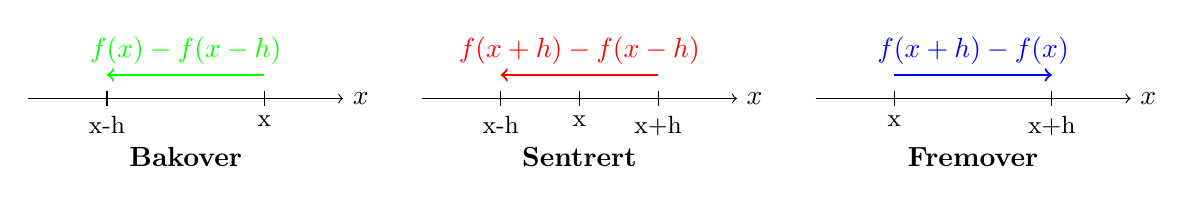
\begin{tikzpicture}
		% Backward Difference Scope
		\begin{scope}[xshift=-5cm]
			\draw[->] (-1,0) -- (3,0) node[right] {$x$}; % Number Line
			\foreach \x/\label in {0/$x-h$, 2/$x$} {
					\draw (\x,0.1) -- (\x,-0.1); % Points
					\node[below] at (\x,-0.1) {\small $\label$}; % Labels
				}
			\draw[->, thick, green] (2,0.3) -- (0,0.3) node[midway, above] {$f(x) - f(x-h)$}; % Arrow for difference
			\node[below] at (1, -0.5) {\textbf{Bakover}}; % Label
		\end{scope}

		% Central Difference Scope
		\begin{scope}[xshift=0cm]
			\draw[->] (-1,0) -- (3,0) node[right] {$x$};
			\foreach \x/\label in {0/$x-h$, 1/$x$, 2/$x+h$} {
					\draw (\x,0.1) -- (\x,-0.1); % Points
					\node[below] at (\x,-0.1) {\small $\label$};
				}
			\draw[->, thick, red] (2,0.3) -- (0,0.3) node[midway, above] {$f(x+h) - f(x-h)$};
			\node[below] at (1, -0.5) {\textbf{Sentrert}};
		\end{scope}

		% Forward Difference Scope
		\begin{scope}[xshift=5cm]
			\draw[->] (-1,0) -- (3,0) node[right] {$x$};
			\foreach \x/\label in {0/$x$, 2/$x+h$} {
					\draw (\x,0.1) -- (\x,-0.1);
					\node[below] at (\x,-0.1) {\small $\label$};
				}
			\draw[->, thick, blue] (0,0.3) -- (2,0.3) node[midway, above] {$f(x+h) - f(x)$};
			\node[below] at (1, -0.5) {\textbf{Fremover}};
		\end{scope}
	\end{tikzpicture}
	\caption{Finite Difference Stencils: Backward, Central, and Forward Difference}
	\label{fig:finite-differences}
\end{figure}


Som figuren viser, benytter \textbf{fremover}-differanser hovedsakelig punkter \emph{til høyre} for \(x_i\),
\textbf{bakover}-differanser benytter hovedsakelig punkter \emph{til venstre} for \(x_i\),
mens \textbf{sentrerte}-differanser er symmetriske rundt \(x_i\).


\section*{Endelig differanseskjema}

Endelige differanseformler gir diskrete tilnærminger av deriverte ved å bruke funksjonsverdier i strategisk utvalgte punkter (ofte kalt \emph{stencil}).
Kolonnene merket \(\mathbf{-3}\) til \(\mathbf{+3}\) (eller flere, avhengig av formelens bredde) oppgir \emph{dimensjonsløse koeffisienter} som multipliserer funksjonsverdiene i \(x_{i + k}\).

For å beregne den deriverte numerisk, må du så dividere med \(h^n\), der \(n\) er den deriverteordenen:

\[
	\frac{d^n f}{dx^n} \Bigg|_{x_i} \approx \frac{1}{h^n} \sum_{k=-m}^{m} \bigl( c_k f(x_{i+k}) \bigr)
\]

\begin{itemize}
	\item \(m\) er halvparten av stencilens bredde (f.eks. 3 for en 7-punkts stencil).
	\item \(c_k\) er dimensjonsløse koeffisienter.
\end{itemize}

\begin{table}[H]
	\centering
	\caption{Finite Difference Coefficients for Various Orders of Accuracy}
	\begin{tabular}{llrrrrrrrl}
		\toprule
		\multirow{2}{*}{Order} & \multirow{2}{*}{Type} & \multicolumn{7}{c}{Coefficients at Position} & \multirow{2}{*}{Error} \\
		\cmidrule{3-9}
		& & \textbf{-3} & \textbf{-2} & \textbf{-1} & \textbf{0} & \textbf{+1} & \textbf{+2} & \textbf{+3} & \\
		\midrule
		\multirow{3}{*}{First} & Forward & & & & -1 & 1 & & & $O(h)$ \\
		& Central & & & -1/2 & 0 & 1/2 & & & $O(h^2)$ \\
		& Backward & & & -1 & 1 & & & & $O(h)$ \\
		\midrule
		\multirow{3}{*}{Higher} & Forward & & & & -3/2 & 2 & -1/2 & & $O(h^2)$ \\
		& Central & & -1/12 & 2/3 & 0 & -2/3 & 1/12 & & $O(h^4)$ \\
		& Backward & & & 1/2 & -2 & 3/2 & & & $O(h^2)$ \\
		\midrule
		\multirow{3}{*}{Second} & Forward & & & & 1 & -2 & 1 & & $O(h^2)$ \\
		& Central & 1/12 & -2/3 & 0 & 2/3 & -1/12 & & & $O(h^4)$ \\
		& Backward & & & 1 & -2 & 1 & & & $O(h^2)$ \\
		\bottomrule
	\end{tabular}
	\label{tab:fd-coefficients}
\end{table}

\begin{example}{}{}
  Hvis vi ønsker å bruke en fremover differanseformel for den første deriverte med $O(h^3)$ nøyaktighet, kan vi bruke koeffisientene fra tabellen: \( \{-11, 18, -9, 2\} \).
  
  Dette gir oss:
  \begin{align*}
    \frac{d}{dx} f(x) & \approx \frac{1}{h} \left( -11f(x) + 18f(x+h) - 9f(x+2h) + 2f(x+3h) \right) \\
                     & = \frac{-11f(x) + 18f(x+h) - 9f(x+2h) + 2f(x+3h)}{h}
  \end{align*}

  For en fremover differanseformel av den andre deriverte med $O(h^2)$ nøyaktighet kan vi bruke koeffisientene: \(\{2, -5, 4, -1\}\).
  
  \medskip
  
  Dette gir oss:
  \begin{align*}
    \frac{d^2}{dx^2} f(x) & \approx \frac{1}{h^2} \left( 2f(x) - 5f(x+h) + 4f(x+2h) - f(x+3h) \right) \\
                         & = \frac{2f(x) - 5f(x+h) + 4f(x+2h) - f(x+3h)}{h^2}
  \end{align*}
\end{example}

\vspace{1em}

\noindent\textbf{Tips for bruk:}
\begin{itemize}
	\item Kontroller alltid \emph{tegnkonvensjon og indeksering} \(\;f(x_{i+k}) \leftrightarrow \text{koeffisient under kolonne }k\).
	\item Etter at koeffisientene er multiplisert med funksjonsverdiene, \emph{deler med} \(h^n\) for en \(n\)-te deriverte.
	\item Fremover/bakover brukes ofte nær kantene av et domene for å unngå ute-av-rekkevidde-punkter.
	\item Sentrerte differanser gir vanligvis høyere nøyaktighet enn fremover- eller bakoverdifferanser, siden de utnytter symmetrien rundt punktet ved å bruke naboverdier likt på begge sider.
\end{itemize}

\section{CFL-betingelsen (Courant-Friedrichs-Lewy)}

CFL-betingelsen er et nødvendig kriterium for stabilitet i tidsdiskretiseringer av hyperbolske og parabolske \gls{pde}. Betingelsen sikrer at det numeriske domenet av avhengighet inkluderer det fysiske domenet av avhengighet.

\begin{definition}{Courant-tall}{courant_number}
	Courant-tallet er definert som:
	\begin{equation}
		C = \frac{u \Delta t}{\Delta x}
	\end{equation}
	der $u$ er bølgehastigheten, $\Delta t$ er tidssteget, og $\Delta x$ er romsteget.
\end{definition}

\subsection{CFL-betingelser for ulike ligninger og skjemaer}

\begin{table}[H]
	\centering
	\caption{CFL-betingelser for ulike typer differensialligninger og numeriske skjemaer}
	\begin{tabular}{lllll}
		\toprule
		\textbf{Ligning} & \textbf{Skjema} & \textbf{CFL-betingelse} & \textbf{Kommentar} & \textbf{Stabilitet} \\
		\midrule
		\multirow{4}{*}{Adveksjon} & FTCS & $C \leq 1$ & $C = \frac{u\Delta t}{\Delta x}$ & Betinget stabil \\
		& Upwind (fremover) & $C \leq 1$ & $C = \frac{|u|\Delta t}{\Delta x}$ & Betinget stabil \\
		& Lax-Wendroff & $C \leq 1$ & $C = \frac{|u|\Delta t}{\Delta x}$ & Betinget stabil \\
		& Implisitt & Ingen & - & Ubetinget stabil \\
		\midrule
		\multirow{4}{*}{Diffusjon} & Eksplisitt & $r \leq \frac{1}{2}$ & $r = \frac{D\Delta t}{(\Delta x)^2}$ & Betinget stabil \\
		& Implisitt (BTCS) & Ingen & - & Ubetinget stabil \\
		& Crank-Nicolson & Ingen & - & Ubetinget stabil \\
		& DuFort-Frankel & $r < \frac{1}{2\mu}$ & $\mu = \sin^2\frac{\pi\Delta x}{\lambda_{min}}$ & Betinget stabil \\
		\midrule
		\multirow{3}{*}{Bølge} & Eksplisitt & $C \leq 1$ & $C = \frac{c\Delta t}{\Delta x}$ & Betinget stabil \\
		& Implisitt & Ingen & - & Ubetinget stabil \\
		& Leapfrog & $C \leq 1$ & $C = \frac{c\Delta t}{\Delta x}$ & Betinget stabil \\
		\midrule
		\multirow{3}{*}{Konveksjon-diffusjon} & Eksplisitt & $C \leq 1, r \leq \frac{1}{2}$ & Begge må oppfylles & Betinget stabil \\
		& FTCS & $r \leq \frac{1}{2}, P_e \leq 2$ & $P_e = \frac{|u|\Delta x}{D}$ & Betinget stabil \\
		& Upwind & $C \leq 1$ & - & Betinget stabil \\
		\midrule
		\multirow{2}{*}{2D Adveksjon} & Eksplisitt & $C_{2D} \leq 1$ & $C_{2D} = \Delta t \left( \frac{|u_x|}{\Delta x} + \frac{|u_y|}{\Delta y} \right)$ & Betinget stabil \\
		& Alternativt vilkår & $C_{alt} \leq 1$ & $C_{alt} = \Delta t \sqrt{ \frac{u_x^2}{\Delta x^2} + \frac{u_y^2}{\Delta y^2} }$ & Betinget stabil \\
		\midrule
		\multirow{2}{*}{2D Diffusjon} & Eksplisitt & $r_{2D} \leq \frac{1}{4}$ & $r_{2D} = D\Delta t \left( \frac{1}{(\Delta x)^2} + \frac{1}{(\Delta y)^2} \right)$ & Betinget stabil \\
		& Alternativt vilkår & $r_{alt} \leq \frac{1}{2d}$ & $d$ = antall dimensjoner & Betinget stabil \\
		\bottomrule
	\end{tabular}
	\label{tab:cfl-conditions}
\end{table}

\subsection{Fysisk tolkning av CFL-betingelsen}

\begin{itemize}
	\item $C < 1$: Informasjon reiser mindre enn én celle per tidssteg (sikker)
	\item $C = 1$: Informasjon reiser nøyaktig én celle per tidssteg (grensetilfelle)
	\item $C > 1$: Informasjon reiser mer enn én celle per tidssteg (ustabilt)
\end{itemize}

\begin{figure}[H]
	\centering
	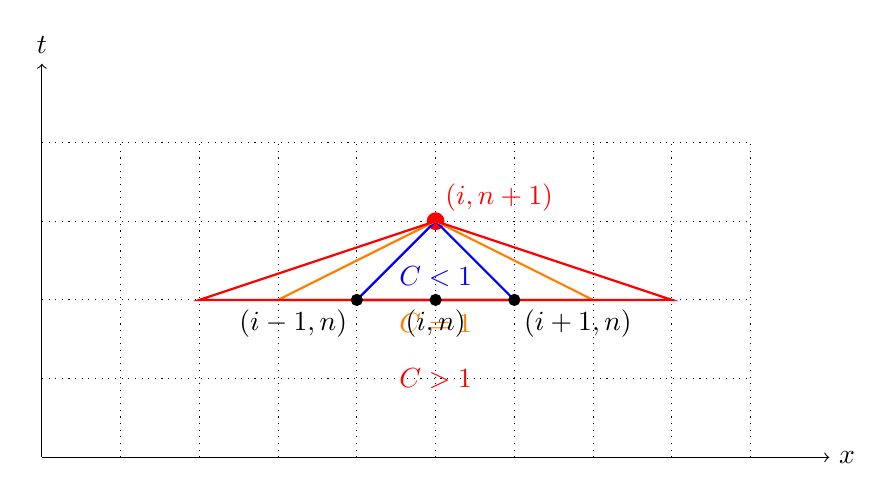
\begin{tikzpicture}
		% Tidsaksen
		\draw[->] (0,0) -- (10,0) node[right] {$x$};
		\draw[->] (0,0) -- (0,5) node[above] {$t$};
		
		% Rutenett
		\foreach \x in {1,2,...,9}
		\draw[dotted] (\x,0) -- (\x,4);
		\foreach \y in {1,2,...,4}
		\draw[dotted] (0,\y) -- (9,\y);
		
		% Punkt hvor vi beregner løsningen
		\filldraw[red] (5,3) circle (3pt);
		\node[red, above right] at (5,3) {$(i,n+1)$};
		
		% Domene av avhengighet i stabil situasjon (C < 1)
		\draw[blue, thick] (5,3) -- (4,2) -- (6,2) -- cycle;
		\node[blue] at (5,2.3) {$C < 1$};
		
		% Domene av avhengighet i grensetilfelle (C = 1)
		\draw[orange, thick] (5,3) -- (3,2) -- (7,2) -- cycle;
		\node[orange] at (5,1.7) {$C = 1$};
		
		% Domene av avhengighet i ustabil situasjon (C > 1)
		\draw[red, thick] (5,3) -- (2,2) -- (8,2) -- cycle;
		\node[red] at (5,1) {$C > 1$};
		
		% Punkter som brukes i beregningen
		\filldraw[black] (4,2) circle (2pt);
		\filldraw[black] (5,2) circle (2pt);
		\filldraw[black] (6,2) circle (2pt);
		\node[below left] at (4,2) {$(i-1,n)$};
		\node[below] at (5,2) {$(i,n)$};
		\node[below right] at (6,2) {$(i+1,n)$};
	\end{tikzpicture}
	\caption{Illustrasjon av CFL-betingelsen med numeriske og fysiske domener av avhengighet}
	\label{fig:cfl-condition}
\end{figure}

\subsection{Praktiske tilnærminger}

\begin{enumerate}
	\item \textbf{Adaptivt tidssteg:} Beregn tillatt $\Delta t$ for hvert steg basert på gjeldende $\Delta x$ og fysiske parametre.
	
	\item \textbf{Global reduksjon:} Multipliser teoretisk maksimum $\Delta t$ med en sikkerhetsfaktor (typisk $0.8-0.9$).
	
	\item \textbf{Alternative metoder:} Vurder implisitte metoder for problemer med strenge CFL-betingelser.
\end{enumerate}

\begin{example}{Beregning av maksimalt tidssteg}{cfl_example}
	For en adveksjonsligning med $u = 100$ m/s og $\Delta x = 0.01$ m:
	\begin{align*}
		\Delta t &\leq \frac{\Delta x}{|u|} \\
		\Delta t &\leq \frac{0.01}{100} = 0.0001 \text{ s}
	\end{align*}
	Med en sikkerhetsfaktor på $0.9$ vil det praktiske tidssteget bli $\Delta t = 9 \times 10^{-5}$ s.
\end{example}



\section{Finite Element Method (FEM)}

FEM er en numerisk metode for å løse PDE ved å diskretisere domenet i enkle geometriske former (elementer) og tilnærme løsningen med en lineærkombinasjon av basisfunksjoner.

\begin{equation}
    u(x) \approx \sum_{i=1}^N c_i \phi_i(x)
\end{equation}

\subsection*{Betingelser for FEM}

For å bruke FEM til å løse et differensiallikningsproblem, må problemet oppfylle følgende betingelser:

\begin{itemize}
    \item \textbf{Linearitet:} Problemet må være lineært, dvs. ligningene kan uttrykkes som \(\mathcal{L}(u) = f\), hvor \(\mathcal{L}\) er en lineær operator.
    \item \textbf{Kontinuerlig Differensierbar:} Løsningen \( u(x) \) må være kontinuerlig differensierbar i domenet \( \Omega \).
    \item \textbf{Geometrisk Enkelhet:} Domenet \( \Omega \) bør kunne deles opp i enkle geometriske elementer (f.eks. trekanter, firkanter i 2D, tetraedre i 3D):
          \[
              \Omega = \bigcup_{e=1}^{E} \Omega_e
          \]
    \item \textbf{Kvantiserbarhet:} Problemet må være kvantiserbart, dvs. løsningen kan tilnærmes godt ved hjelp av en endelig basisfunksjon:
          \[
              u_h(x) = \sum_{i=1}^{N} c_i \phi_i(x)
          \]
    \item \textbf{Randbetingelser:} Randbetingelsene må være kompatible med valg av funksjonsrom:
          \[
              u|_{\partial \Omega} = g \quad \text{eller} \quad \frac{\partial u}{\partial n}\bigg|_{\partial \Omega} = h
          \]
\end{itemize}

\subsection*{FEM-oppskrift}

\begin{enumerate}
    \item \textbf{Diskretisering:} Del domenet \( \Omega \) inn i enkle geometriske elementer \( \Omega_e \) og tilnærme løsningen med en lineærkombinasjon av basisfunksjoner:
          \[
              u(x) \approx \sum_{i=1}^N c_i \phi_i(x)
          \]
    \item \textbf{Svak formulering:} Multipliser differensiallikningen med en testfunksjon \( v(x) \) og integrer over domenet \( \Omega \):
          \[
              \int_\Omega v(x) \mathcal{L}(u) \, dx = \int_\Omega v(x) f(x) \, dx
          \]

    \item \textbf{Galerkin-prosedyre:} Tilnærme løsningen og testfunksjonen med basisfunksjoner:
            \[
                u(x) \approx \sum_{i=1}^N c_i \phi_i(x) \quad \text{og} \quad v(x) \approx \sum_{j=1}^N d_j \phi_j(x)
            \]
    \item \textbf{Diskretisering:} Set inn tilnærmingene i den svake formen og diskretiser:
          \[
              \sum_{j=1}^N d_j \int_\Omega \phi_j(x) \mathcal{L} \left( \sum_{i=1}^N c_i \phi_i(x) \right) \, dx = \sum_{j=1}^N d_j \int_\Omega \phi_j(x) f(x) \, dx
          \]
    \item \textbf{Matriseform:} Skriv den diskretiserte formen som et ligningssett \( A\vec{c} = \vec{b} \) og løs for koeffisientene \( \vec{c} \).
\end{enumerate}


\begin{definition}{Viktige definisjoner for FEM}{}
    \begin{enumerate}
        \item \textbf{Skalarprodukt} \(\langle v, w \rangle\): Integral av produktet av to funksjoner over domenet \(\Omega\):
              \[ \langle v, w \rangle = \int_\Omega v(x)w(x) \, dx \]
              ofte er \(\Omega := (0,1)\).
        \item \textbf{Funksjonsrommet} \(V\): Rommet av funksjoner som tilfredsstiller randbetingelsene.

              \[ V = \{ v \in C^2(\Omega) \, | \, v(a) = \alpha, v(b) = \beta \} \]

        \item \textbf{Testfunksjoner} \(v(x)\): Funksjoner i \(V\) som brukes til å formulere den svake formen.
        \item \textbf{Basisfunksjoner} \(\phi_i(x)\): Lokale funksjoner som spenner ut løsningsrommet.
              \begin{itemize}
                  \item Har kompakt støtte (er null utenfor et lite område)
                  \item Oppfyller \(\phi_i(x_j) = \delta_{ij}\) (Kronecker delta)
              \end{itemize}
        \item \textbf{Energifunksjon} \(F(v) = \frac{1}{2} \langle v, v \rangle - \langle f, v \rangle\): Energien til en funksjon \(v\). Kan intuitivt tolkes som en måling av hvor mye energi som kreves for å produsere \(v\).
    \end{enumerate}
\end{definition}

Først trenger vi å formulere problemet. f.eks. for en Poisson-ligning:
\begin{equation}
    \begin{cases}
        -\ddn[2]{u(x)}{x} = f(x),  & x \in (0,1)              \\
        u(0) = \alpha, \quad u(1) = \beta & \text{(randbetingelser)}
    \end{cases}
    \label{eq:pde_poisson}
\end{equation}

\begin{equation}
    \mathbf{F} = - \int_0^1 f(x) \mathbf{N}(x) dx
\end{equation}

La \(f(x) = \bar{f}\) være konstant.

\begin{equation*}
    \mathbf{F} = - \bar{f} \int_0^1 \mathbf{N}(x) dx = - \bar{f} \begin{bmatrix}
        0.1 \\ 0.2 \\ 0.2 \\ 0.2 \\ 0.2 \\ 0.1
    \end{bmatrix}
\end{equation*}


\subsection{Lecture 8 (28.1.2025)}

\begin{theorem}{Lax-Equivalence-Theorem}{}
    \[
        \text{Consistency} + \text{Stability} \iff \text{Convergence}
    \]
    Holds for linear (time-dependent) problems.
\end{theorem}

PDE:

\begin{align*}
    u_t + u_x  = au, \quad \R \\
    u(x, 0) = f(x) \tag{IC}   \\
    u(0, t) = g(t) \tag{BC}   \\
    u(x,t) =
    \begin{cases}
        e^{at}f(x-t), & x < t \\
        e^{at}g(t-x), & x > t
    \end{cases}
\end{align*}

\paragraph{Scheme:}
\begin{align*}
    U_m^{n+1} = U_m^n - \frac{K}{h}(U_m^n - U_{m-1}^n) + aKU_m^n \\
    \tau_m^n = \frac{1}{2}(K\partial_t^2 u_m^n - h\partial_x^2 u_m^n) + O(K^2 + h^2)
\end{align*}

\[
    \norm{\vec{\tau}^n} \underset{h, K \to 0}{\longrightarrow} 0 \tag{Consistency}
\]

\paragraph{Stencil:}
\begin{figure}[H]
    \centering
    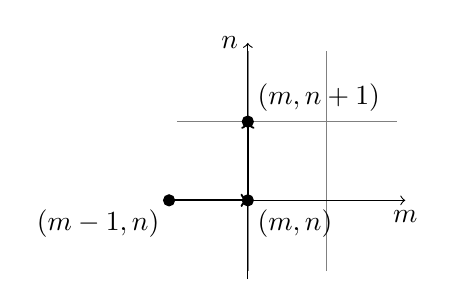
\begin{tikzpicture}
        \draw[step=1cm,gray,very thin] (-0.9,-0.9) grid (1.9,1.9);
        \draw[->] (-1,0) -- (2,0) node[below] {$m$};
        \draw[->] (0,-1) -- (0,2) node[left] {$n$};
        \filldraw[black] (0,0) circle (2pt) node[below right] {$(m,n)$};
        \filldraw[black] (-1,0) circle (2pt) node[below left] {$(m-1,n)$};
        \filldraw[black] (0,1) circle (2pt) node[above right] {$(m,n+1)$};
        \draw[->,thick] (0,0) -- (0,1);
        \draw[->,thick] (-1,0) -- (0,0);
    \end{tikzpicture}
    \caption{Stencil}
    \label{fig:stencil}
\end{figure}

\paragraph{Stability:}
Find \(C\). Define \( S = \frac{K}{h} \).

\[
    U_m^{n+1} = (1 - S + aK)U_m^n + SU_{m-1}^n
\]

\[
    \begin{bmatrix}
        U_1^{n+1} \\
        U_2^{n+1} \\
        \\
        \vdots    \\
        \\
        U_M^{n+1}
    \end{bmatrix}
    =
    \begin{bmatrix}
        1 - S + aK & 0          & 0          & \cdots & 0          \\
        S          & 1 - S + aK & 0          & \cdots & 0          \\
        0          & S          & 1 - S + aK & \cdots & 0          \\
        \vdots     & \vdots     & \vdots     & \ddots & \vdots     \\
        0          & \cdots     & 0          & S      & 1 - S + aK
    \end{bmatrix}
    \begin{bmatrix}
        U_1^n  \\
        U_2^n  \\
        \\
        \vdots \\
        \\
        U_M^n
    \end{bmatrix}
    +
    \begin{bmatrix}
        \overbrace{S g(t_0)}^{U_0^n} \\
        0                            \\
        \vdots                       \\
        0                            \\
        \overbrace{S g(t_n)}^{U_{M+1}^n}
    \end{bmatrix}
\]

\begin{example}{}{}
    \begin{align*}
        u_t = u_{xx} \text{ on } [0,1] \\
        u(x, 0) = f(x)                 \\
        u(1, t) = 0                    \\
        u(0, t) + u_x(0, t) = 0
    \end{align*}
    \paragraph{Scheme}
    let \( r= \frac{K}{h^2} \)
    \[
        U_m^{n+1} = U_m^n + r(U_{m-1}^n - 2U_m^n + U_{m+1}^n)
    \]
    \paragraph{Boundary Conditions}
    \begin{align*}
        U_0^{n+1} = U_0^n + r(U_1^n - 2U_0^n + U_{-1}^n)        \\
        U_0^n + \frac{1}{2h}(U_1^n - U_{-1}^n) = 0              \\
        U_{-1}^n = U_1^n + 2hU_0^n                              \\
        U_0^{n+1} = U_0^n + r(U_1^n - 2U_0^n + U_1^n + 2hU_0^n) \\
        U_0^{n+1} = U_0^n + r(2U_1^n - 4U_0^n)                  \\
        U_0^{n+1} = U_0^n + 2rU_1^n - 4rU_0^n                   \\
        U_0^{n+1} = (1 - 2r(1 - h))U_0^n + 2rU_1^n
    \end{align*}
    Let \( \vec{U}^n = \begin{bmatrix} U_0^n \\ U_1^n \\ \vdots \\ U_M^n \end{bmatrix} \) where \( U_M^n = 0 \).

    \[
        C = \begin{bmatrix}
            1 - 2r(1 - h) & 2r     & 0      & \cdots & 0      \\
            r             & 1 - 2r & r      & \cdots & 0      \\
            0             & r      & 1 - 2r & \cdots & 0      \\
            \vdots        & \vdots & \vdots & \ddots & \vdots \\
            0             & \cdots & 0      & r      & 1 - 2r
        \end{bmatrix}
    \]

    Need to find \( r \leq \frac{1}{2} \) for \(m = 1, 2, \ldots, M-1\) to ensure stability.
    For \( m = 0 \) we need:
    \begin{align*}
        \abs{1 - 2r(1 - h)} + \abs{2r} \leq 1 + \mu K \\
        \abs{1 - 2r(1 - h)} + 2r \leq \abs{1 - 2r} + 2rh + \abs{2r} = 1 + 2rh = 1 + \underbrace{\frac{2}{h}}_{\mu}K
    \end{align*}
    Stable for a given \( h \) but not when \( h \to 0 \).
    \begin{align*}
        K \tau_0^n =                              & u(0, t_n + h) - u(0, t_n) + 2r(1 - h)u(0, t_n) - 2ru(h, t_n)                                                                                                                                            \\                                                                                                                                                                                                                    \\
        =            u_0^n + K \partial_t u_0^n + & \frac{1}{2}K^2 \partial_t^2 u_0^n + \ldots - u_0^n                                                                                                                                                      \\
        +                                         & 2\frac{K}{h^2}(1 - h)u_0^n - 2\frac{K}{h^2}(u_0^n + h \partial_x u_0^n + \frac{1}{2}h^2 \partial_x^2 u_0^n + \frac{1}{6}h^3 \partial_x^3 u_0^n + \frac{1}{24}h^4 \partial_x^4 u_0^n + \ldots)           \\
                                                  & = \frac{K}{h^2}\left[-h(u_0^n + \partial_x u_0^n)\right] + K \left[\partial_t u_0^n - \partial_x^2 u_0^n\right] - \frac{1}{3}Kh\partial_x^3 u_0^n + \ldots + \frac{1}{2}K^2 \partial_t^2 u_0^n + \ldots \\
        K \tau_0^n                                & = -\frac{1}{3}Kh\partial_x^3 u_0^n + \ldots + \frac{1}{2}K^2 \partial_t^2 u_0^n + \ldots \tag{Consistency}
    \end{align*}
\end{example}

\subsection*{Alternative stability analysis: Von Neumann analysis}
Von Neumann analysis is a method for analyzing the stability of finite difference schemes for linear partial differential equations.
The method is based on the Fourier analysis of the numerical solution.

\begin{theorem}{Parseval's equality}{}
    \[
        \sum_{l=-\infty}^{\infty} \abs{C_l}^2 = \frac{1}{2\pi} \int_0^{2\pi} \abs{f(x)}^2 \dd{x}
    \]
\end{theorem}

\begin{example}{}{}
    \begin{align*}
        u_t = u_{xx} \text{ on } [0,1] \\
        u(x, 0) = f(x)                 \\
    \end{align*}
    Make a periodic extension of \(f\), s.t. \(f(x) = f(x-1)\).
    Assue that \(u(x-1, t) = u(x, t)\) and \(u(1, t) = u(0, t)\).
    Write \(f(x)\) as a complex Fourier series:
    \begin{align*}
        f(x) & = \sum_{k=-\infty}^{\infty} C_l e^{i \beta_l x}, \quad \beta_l = 2\pi l, \quad l \in \Z \\
        C_l  & = \int_0^1 f(x) e^{-i \beta_l x} \dd{x}
    \end{align*}

    Seperation of variables:
    \[
        u_l(x, t) = e^{-\beta_l^2 t} e^{i \beta_l x}
    \]
    Plug in the (IC):
    \[
        u(x, t) = \sum_{l=-\infty}^{\infty} C_l e^{-\beta_l^2 t} e^{i \beta_l x}
    \]
    \subparagraph{Idea}
    Given a scheme for \(u_t = u_{xx}\), we can write:
    \[
        U_m^{n+1} = U_m^n + r(U_{m-1}^n - 2U_m^n + U_{m+1}^n), \quad r = \frac{k}{h^2}
    \]

    Search for a solution of the form:
    \[
        U_m^n = \psi^n e^{i \beta x_m}
    \]
    A scheme is \textit{Von Neumann stable} if:
    \[
        \abs{\psi} < 1 + \mu k, \quad \mu \geq 0
    \]

    In our example:
    \begin{align*}
        \psi^{n+1} e^{i \beta x_m} & = \psi^n e^{i \beta x_m} + r\psi^n\left(e^{i \beta x_{m+1}} - 2e^{i \beta x_m} + e^{i \beta x_{m-1}}\right) \\
                                   & = \psi^n e^{i \beta x_m} (1 + r(e^{i \beta h} - 2 + e^{-i \beta h}))                                        \\
        \psi                       & = 1 + r(e^{i \beta h} - 2 + e^{-i \beta h})                                                                 \\
                                   & = 1 + r(2\cos(\beta h) - 2)                                                                                     \\
                                      & = 1 + 4r\sin^2\left(\frac{\beta h}{2}\right)                                                                    \\
        \abs{\psi}                 & = \abs{1 + 4r\sin^2\left(\frac{\beta h}{2}\right)} \leq 1 \iff r \leq \frac{1}{2}, \forall \beta \text{ and } \mu = 0
    \end{align*}
\end{example}

\section{Forelesninger}

\input{sections/lectures/lecture8.tex}
\subsection{Mandag \date{3. februar 2025}}

\paragraph{Von Neumann Stability Analysis}
\begin{itemize}
  \item Let \( U_m^n = \xi^n e^{i\beta m} \). Insert this into Difference Equation (DE).
  \item The method is Von Neumann Stable if \( \abs{\xi} \leq 1 + \mu K \) for all \( \beta \).
  \item Von Neumann stability is sufficient and necessary for pure IVP problems (Cauchy problems).
\end{itemize}
\begin{figure}[H]
  \centering
  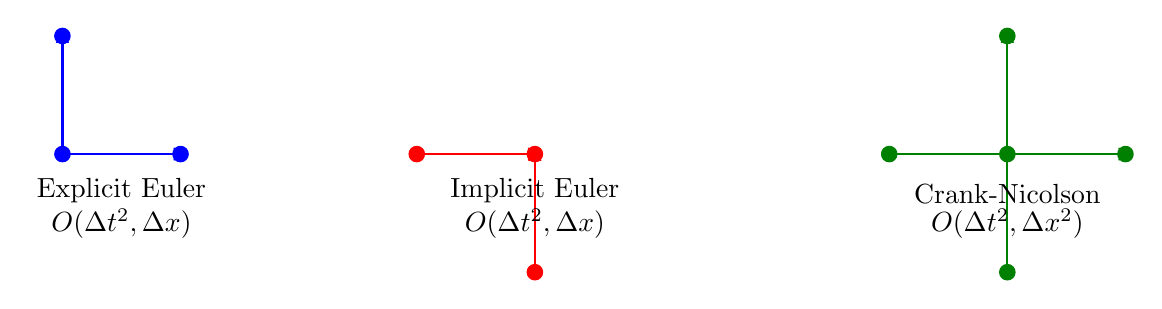
\begin{tikzpicture}[scale=1.5]
    % Explicit Euler (Forward)
    \begin{scope}[xshift=0cm]
      \fill[blue] (0,0) circle (2pt);
      \fill[blue] (0,1) circle (2pt);
      \fill[blue] (1,0) circle (2pt);
      \draw[->,thick,blue] (0,0) -- (1,0);
      \draw[->,thick,blue] (0,0) -- (0,1);
      \node[above] at (0.5,-0.5) {Explicit Euler};
      \node[above] at (0.5,-0.8) {$O(\Delta t^2, \Delta x)$};
    \end{scope}

    % Implicit Euler (Backward)
    \begin{scope}[xshift=4cm]
      \fill[red] (0,0) circle (2pt);
      \fill[red] (-1,0) circle (2pt);
      \fill[red] (0,-1) circle (2pt);
      \draw[->,thick,red] (-1,0) -- (0,0);
      \draw[->,thick,red] (0,-1) -- (0,0);
      \node[above] at (0,-0.5) {Implicit Euler};
      \node[above] at (0,-0.8) {$O(\Delta t^2, \Delta x)$};
    \end{scope}

    % Crank-Nicolson
    \begin{scope}[xshift=8cm]
      \fill[green!50!black] (0,0) circle (2pt);
      \fill[green!50!black] (1,0) circle (2pt);
      \fill[green!50!black] (-1,0) circle (2pt);
      \fill[green!50!black] (0,1) circle (2pt);
      \fill[green!50!black] (0,-1) circle (2pt);
      \draw[->,thick,green!50!black] (-1,0) -- (1,0);
      \draw[->,thick,green!50!black] (0,-1) -- (0,1);
      \node[above] at (0,-0.5) {Crank-Nicolson};
      \node[above] at (0,-0.8) {$O(\Delta t^2, \Delta x^2)$};
    \end{scope}
  \end{tikzpicture}
  \caption{Stencils for different numerical schemes}
  \label{fig:stencils}
\end{figure}



\begin{example}{Heat equation}{}
  \[
    u_t = u_{xx}, \quad 0 \leq x \leq 1, \quad 0 \leq t \leq 0.5
  \]
  \[
    \begin{cases}
      u(x, 0) = \sin(\pi x) \\
      u(0, t) = u(1, t) = 0
    \end{cases}
  \]
  \[
    u(x, t) = \sin(\pi x) e^{-\pi^2 t}
  \]

  \subparagraph{Finite Difference Scheme}
  \[
    \frac{1}{2k}\left( U_m^{n+1} - U_m^{n-1} \right) = \frac{1}{h^2}\left( U_{m-1}^n - 2U_m^n + U_{m+1}^n \right)
  \]

  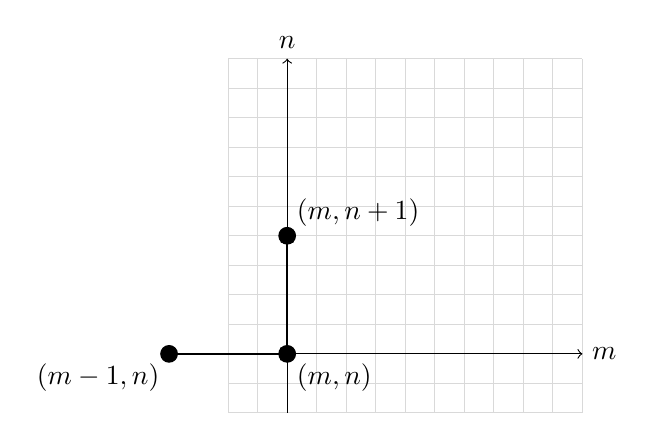
\begin{tikzpicture}[scale=1.5]
    % Grid
    \draw[step=0.25cm,gray!30] (-0.5,-0.5) grid (2.5,2.5);
    \draw[->] (-0.5,0) -- (2.5,0) node[right] {$m$};
    \draw[->] (0,-0.5) -- (0,2.5) node[above] {$n$};
    % Points
    \filldraw[black] (0,0) circle (2pt) node[below right] {$(m,n)$};
    \filldraw[black] (-1,0) circle (2pt) node[below left] {$(m-1,n)$};
    \filldraw[black] (0,1) circle (2pt) node[above right] {$(m,n+1)$};
    % Arrows
    \draw[->,thick] (0,0) -- (0,1);
    \draw[->,thick] (-1,0) -- (0,0);

  \end{tikzpicture}


  \subparagraph{Fourier Stability Analysis}

  \begin{align*}
    U_m^{n+1}
     & =
    2r\left( U_{m-1}^n - U_m^n + U_{m+1}^n \right) + U_m^{n-1}               \\
    \xi^{n+1} e^{i\beta x_m}
     & =
    2r\xi^n
    \left[
      e^{i\beta x_m - h} - 2e^{i\beta x_m} + e^{i\beta x_m + h}
      \right]
    + \xi^{n-1} e^{i\beta x_m}                                               \\
    \xi^2
     & =
    2r\left[ e^{-i\beta h} - 2 + e^{i\beta h} \right]\xi + 1                 \\
    \xi^2
     & =
    2r \left[ 2\cos(\beta h) - 2 \right]\xi+ 1                               \\
    \xi^2 + 8r\sin^2 \frac{\beta h}{2}\xi - 1
     & =
    0 \quad  \implies \quad \xi_\pm
    =
    -4r\sin^2 \frac{\beta h}{2} \pm \sqrt{16r^2\sin^4 \frac{\beta h}{2} + 1} \\
    \xi_- \leq - 1
    \quad
    \abs{\xi_-} \leq 1
  \end{align*}

  \textbf{Conclusion:} The scheme is unconditionally unstable.

  But we can stabilize the scheme by introducing a damping term (Du Fort-Frankel scheme):
  Replace \( U_m^n \leftarrow \frac{1}{2}(U_m^{n+1} + U_m^{n-1}) \) in the scheme.

  \begin{align*}
    \frac{1}{2k}\left( U_m^{n+1} - U_m^{n-1} \right)
     & =
    \frac{1}{h^2}\left( U_{m-1}^n + U_{m+1}^n\right) - \frac{1}{h^2}\left( U_m^{n+1} + U_m^{n-1} \right) \\
    (1 + 2r)U_m^{n+1}
     & =
    2r\left( U_{m-1}^n + U_{m+1}^n \right) + (1 - 2r)U_m^{n-1}                                           \\
    (1 + 2r)\xi^2 - 4r \cos \beta h \xi - (1 - 2r)
     & = 0                                                                                               \\
    \xi_\pm
     & = \frac{1}{1 + 2r} \left[ 2r\cos \beta h \pm \sqrt{4r^2\cos^2 \beta h + (1 - 2r)(1 + 2r)} \right] \\
    \xi_\pm
     & = \frac{1}{1 + 2r} \left[ 2r\cos \beta h \pm \sqrt{1 - 4r^2 \sin^2 {bh}} \right]                  \\
    \abs{\xi_\pm}^2 = \frac{2r - 1}{2r + 1} < 1 \quad \text{for all } r                                  \\
  \end{align*}

  \textbf{Conclusion:} The method scheme is unconditionally stable, for all \( r \).

  Now we know that the scheme has stability for all \( r \), it might still not converge because we also need consistency.

  \subparagraph{Consistency}
  \begin{align*}
    \tau_m^n
     & =
     & \frac{1}{2k}\left( u_m^{n+1} - u_m^{n-1} \right)                                                 \\
     & - \frac{1}{h^2}\left( u_{m-1}^n - u_{m+1}^n \right)                                              \\
     & + \frac{1}{h^2}\left( u_m^{n+1} - u_m^{n-1} \right)                                              \\
     & =
     & \frac{1}{2k}\left[ 2k u_t + 2k^3 \frac{1}{3!}u_{tt} + \ldots \right]                             \\
     & -\frac{1}{h^2}\left[ 2u + 2h^2 \frac{1}{2!}u_{xx} + 2h^4 \frac{1}{4!}u_{xxxx} + \ldots \right]   \\
     & + \frac{1}{h^2}\left[ 2 u + 2k^2 \frac{1}{2!}u_{tt} + 2k^4 \frac{1}{4!}u_{tttt} + \ldots \right] \\
     & =
    u_t - u_xx 
    + \frac{k^2}{h^2}u_{tt} + \frac{k^2}{3!}u_{tt} 
    + \frac{h^2}{12}u_{xxxx} + \frac{k^4}{12h^2}u_{tttt} 
    + \ldots
  \end{align*}
  The method is consistent only if the truncation error goes to zero as \( h, k \to 0 \).

  Here the method is consistent when \(\frac{k}{h} \underset{h,k \to 0}{\longrightarrow} 0\).

  \textbf{Conclusion:} The method is conditionally consistent.

  \textbf{Conclusion:} The method is conditionally stable and consistent for all \( r \) and \( \frac{k}{h} \underset{h,k \to 0}{\longrightarrow} 0 \) and therefore convergent.

\end{example}

\subsection*{Domain of dependence}



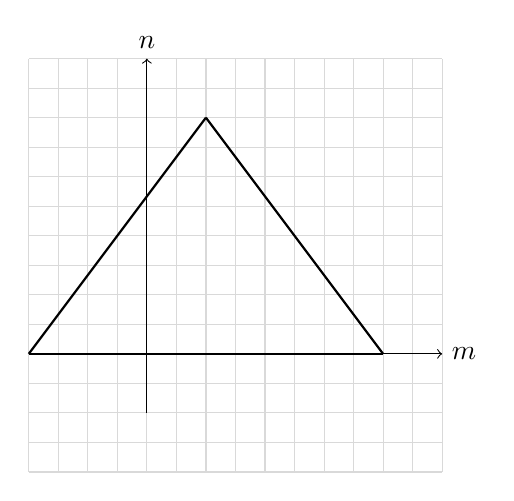
\begin{tikzpicture}[scale=1.5]
  % Grid
  \draw[step=0.25cm,gray!30] (-1,-1) grid (2.5,2.5);
  \draw[->] (-1,0) -- (2.5,0) node[right] {$m$};
  \draw[->] (0,-0.5) -- (0,2.5) node[above] {$n$};

  % Triangle
  \draw[-,thick] (-1,0) -- (0.5,2);
  \draw[-,thick] (-1,0) -- (2,0);
  \draw[-,thick] (2,0) -- (0.5,2);

\end{tikzpicture}




\end{document}